\clearpage
\section{Wertschöpfungskette}
\subsection{Modelle}
\subsubsection{Porter}
Bei dem Modell einer Wertschöpfungskette, wie sie von Michael E. Porter in seinem Buch \emph{Competitive Advantage} beschrieben wurde, dargestellt in Abbildung \ref{fig:porter_00} auf Seite \pageref{fig:porter_00}, setzt sich die Wertgewinnung aus primär- \& sekundär(/support)-Aktivitäten zusammen und mündet in eine Marge.\\
Hierbei erreichen die Primäraktivitäten die eigentliche Wertschöpfung. Sekun-där- bzw. Supportaktivitäten können das nicht. Sie können Primäraktivitäten aber in ihrer Wertschöpfung unterstützen bzw. eine Grundlage für diese bilden.
\begin{figure}[htb]
\centering
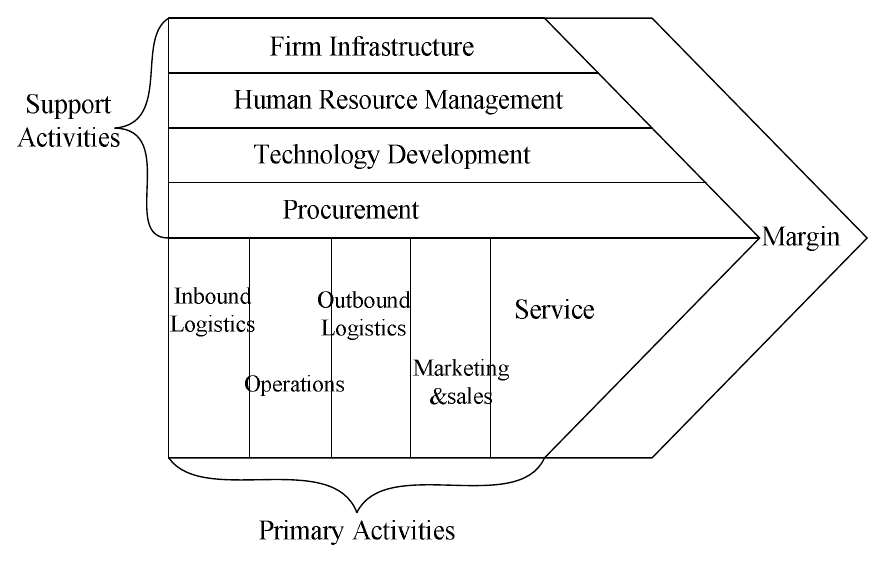
\includegraphics[width=\textwidth]{img/value_chain_porter.png}
\caption{Wertschöpfungskette nach Porter}
\label{fig:porter_00}
\end{figure}
\subsubsection[E-Commerce Wertschöpfungskette]{E-Commerce Wertschöpfungskette\footnote{Mi Yan, "Analysis on Mobile E-Commerce Value-Chain," Management of e-Commerce and e-Government, 2008. ICMECG '08. International Conference on , vol., no., pp.53,56, 17-19 Oct. 2008
doi: 10.1109/ICMECG.2008.43}}
In seinem Paper \emph{Analysis on Mobile E-Commerce Value-Chain} beschreibt Mi Yan ein Modell einer Wertschöpfungskette angelehnt an das Modell von Porter, zu sehen auf Abbildung \ref{fig:ecvc_00} auf Seite \pageref{fig:ecvc_00}. Priäraktivitäten sind hier allerdings \emph{Information}, \emph{Bargaining}, \emph{Transaction}, \emph{Distribution} und \emph{Service}. Anstatt der Sekundäraktivitäten gibt es sogenannte \emph{Operational Modes}: \emph{Organizational Model}, \emph{Operational Model} und \emph{Actual Support}.

.
\begin{figure}[htb]
\centering
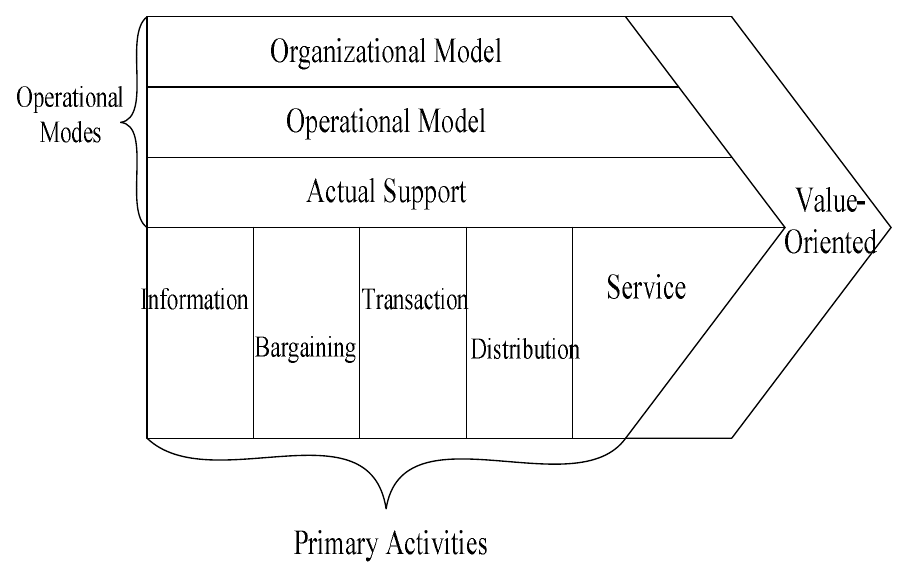
\includegraphics[width=\textwidth]{img/value_chain_ec1.png}
\caption{E-Commerce Wertschöpfungskette nach Mi Yan}
\label{fig:ecvc_00}
\end{figure}

\subsubsection[Einordnung E-Payment in die EC Wertschöpfungskette]{Einordnung E-Payment in die EC Wertschöpfungskette\footnote{A. Meier, H. Stormer, eBusiness \& eCommerce, DOI 10.1007/978-3-642-29802-8\_7,© Springer-Verlag Berlin Heidelberg 2012}}
Ein weiteres Modell bietet die auf Abbildung \ref{fig:ecvc_01} auf Seite \pageref{fig:ecvc_01} dargestellte Einordung des E-Payment in die Wertschöpfungskette des E-Commerce. Hier sehen wir also keine Aufteilung der Wertgewinnung im Bereich E-Payment, sondern einen Blick von Außen, ausgehend von der \emph{E-Society} und die Position des E-Payment innerhalb dieser.
\begin{figure}[htb]
\centering
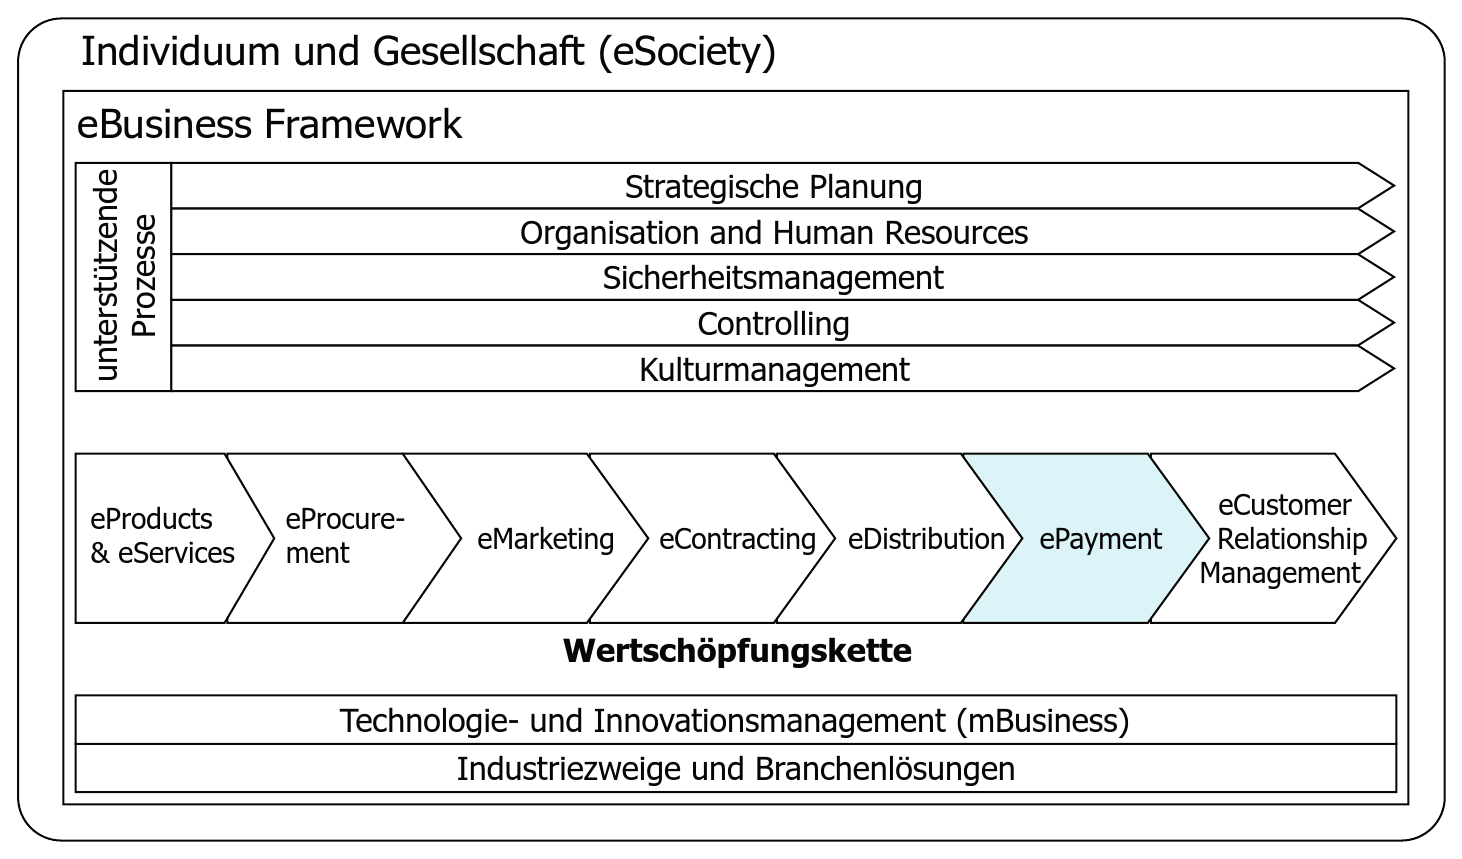
\includegraphics[width=\textwidth]{img/value_chain_ec2.png}
\caption{Einordnung des E-Payment}
\label{fig:ecvc_01}
\end{figure}
\subsection{Analyse}
\textbf{Rayport und Sviokla}\footnote{Rayport, J. F., and Sviokla, J. J. “Exploiting the Virtual Value Chain.” Harvard Business Review (November-December 1995): 75-85.}\\
Bezogen auf Mi Yans E-Commerce Wertschöpfungskette, welche am ehesten den Prozess der Wertgewinnung im Bereich E-Payment darstellt, lässt sich festhalten, dass jede wertschöpfende Aktivität in physische Wertschöpfung (basierend auf materiellen Resourcen, der traditionellen physischen Wert-schöpfungskette) und Werschöpfung basierend auf Information als Rerource (virtuelle Wertschöpfungskette) aufgeteilt werden kann. In letztgenanner spielt Information nicht mehr nur eine unterstützende Rolle sondern aktive Komponente des Wertschöpfungsprozesses.\\
\\
Man kann also aussagen, dass die Wertschöpfung im Bereich E-Commerce sich bedeutend von Porters Modell unterscheidet. Information hat einen deutlich höheren Stellenwert und ist aktiver Teil der Wertschaffung. Anders wäre eine Gewinnerziehlung durch E-Commerce schließlich auch nicht möglich, da nichts Physisches produziert oder an den Kunden vertrieben wird.
